% !TEX program = xelatex
% !TEX encoding = UTF-8 Unicode
\documentclass[11pt,a4paper]{article}

% =========================================================================
% CẤU HÌNH GÓI VÀ FONT HỆ THỐNG
% =========================================================================
\usepackage{fontspec}
\setmainfont{Arial}[
  BoldFont = {arialbd.ttf},
  ItalicFont = {ariali.ttf},
  BoldItalicFont = {arialbi.ttf}
]
\setmonofont{Consolas}[Scale=0.92]

\usepackage[top=20mm, bottom=20mm, left=18mm, right=18mm, headheight=20pt]{geometry}
\usepackage{amsmath, amssymb, amsfonts, bm, mathtools}
\usepackage{booktabs, tabularx, multirow, array, float}
\usepackage{graphicx}
\usepackage{xcolor}
\usepackage{tcolorbox}
\tcbuselibrary{skins, breakable}
\usepackage{fancyhdr}
\usepackage{titlesec}
\usepackage{enumitem}
\usepackage{caption}
\usepackage{listings}

% =========================================================================
% BẢNG MÀU CHUẨN THIẾT KẾ CLASSTWIN
% =========================================================================
\definecolor{NavyDark}{HTML}{0D233A}
\definecolor{NavyBlue}{HTML}{1A365D}
\definecolor{TealPrimary}{HTML}{007A87}
\definecolor{TealLight}{HTML}{E6F4F6}
\definecolor{TealBorder}{HTML}{99D5DC}
\definecolor{SlateGray}{HTML}{4A5568}
\definecolor{MutedGray}{HTML}{718096}
\definecolor{LightBg}{HTML}{F8FAFC}
\definecolor{AccentAmber}{HTML}{D97706}
\definecolor{BorderGray}{HTML}{E2E8F0}
\definecolor{CodeBg}{HTML}{F1F5F9}
\definecolor{CodeKeyword}{HTML}{0F766E}
\definecolor{CodeString}{HTML}{B45309}
\definecolor{CodeComment}{HTML}{64748B}

% =========================================================================
% CẤU HÌNH GÓI LISTINGS
% =========================================================================
\lstdefinelanguage{JavaScript}{
  keywords={typeof, new, true, false, catch, function, return, null, switch, var, if, in, while, do, else, case, break, const, let, async, await, class, export, default, document, window, fetch, Math, Date, performance},
  keywordstyle=\color{CodeKeyword}\bfseries,
  sensitive=true,
  comment=[l]{//},
  morecomment=[s]{/*}{*/},
  commentstyle=\color{CodeComment}\itshape,
  stringstyle=\color{CodeString}\ttfamily,
  morestring=[b]',
  morestring=[b]"
}

\lstdefinelanguage{json}{
  stringstyle=\color{CodeString},
  numbers=left,
  stepnumber=1,
  showstringspaces=false,
  breaklines=true,
  string=[s]{"}{"}
}

\lstset{
  backgroundcolor=\color{CodeBg},
  basicstyle=\ttfamily\footnotesize\color{NavyDark},
  breaklines=true,
  captionpos=b,
  commentstyle=\color{CodeComment}\itshape,
  frame=single,
  framerule=0.5pt,
  rulecolor=\color{BorderGray},
  keepspaces=true,
  keywordstyle=\color{CodeKeyword}\bfseries,
  numbers=left,
  numbersep=6pt,
  numberstyle=\tiny\color{MutedGray},
  showstringspaces=false,
  stringstyle=\color{CodeString},
  tabsize=2
}

% =========================================================================
% CẤU HÌNH HYPERREF
% =========================================================================
\usepackage[
  colorlinks=true,
  linkcolor=NavyBlue,
  citecolor=TealPrimary,
  urlcolor=TealPrimary,
  bookmarks=true,
  bookmarksnumbered=true,
  pdfstartview=FitH,
  pdftitle={ClassTwin - Ke Hoach Demo Trien Khai Telemetry 1, 2, 3, 8},
  pdfauthor={SCIC 2026 Team}
]{hyperref}

% =========================================================================
% HEADER / FOOTER
% =========================================================================
\pagestyle{fancy}
\fancyhf{}
\fancyhead[L]{\textcolor{MutedGray}{\footnotesize \textbf{SCIC 2026} • Kế Hoạch Demo Nền Tảng Viễn Trắc Thực Địa (Nhóm 1, 2, 3, 8)}}
\fancyhead[R]{\textcolor{NavyDark}{\footnotesize \textbf{ClassTwin Prototype}}}
\fancyfoot[L]{\textcolor{MutedGray}{\footnotesize Bản quyền đề án © 2026 ClassTwin Team.}}
\fancyfoot[R]{\textcolor{NavyDark}{\footnotesize \textbf{Trang \thepage}}}
\renewcommand{\headrulewidth}{0.5pt}
\renewcommand{\footrulewidth}{0.4pt}

% =========================================================================
% ĐỊNH DẠNG TIÊU ĐỀ
% =========================================================================
\titleformat{\section}
  {\color{NavyDark}\large\bfseries}
  {\thesection.}{0.6em}{}
  [\color{TealPrimary}\titlerule]

\titleformat{\subsection}
  {\color{TealPrimary}\normalsize\bfseries}
  {\thesubsection}{0.5em}{}

% =========================================================================
% HỘP TCOLORBOX GỌN NHẸ
% =========================================================================
\newtcolorbox{stepbox}[1][]{
  colback=LightBg,
  colframe=TealPrimary,
  fonttitle=\bfseries\color{white},
  coltitle=white,
  boxrule=0.7pt,
  arc=2pt,
  left=8pt, right=8pt, top=6pt, bottom=6pt,
  title={#1},
  breakable
}

\newtcolorbox{alertbox}[1][]{
  colback=LightBg,
  colframe=AccentAmber,
  fonttitle=\bfseries\color{white},
  coltitle=white,
  boxrule=0.7pt,
  arc=2pt,
  left=8pt, right=8pt, top=6pt, bottom=6pt,
  title={#1},
  breakable
}

\setlist[itemize]{leftmargin=1.3em, itemsep=1.5pt, topsep=2pt}
\setlist[enumerate]{leftmargin=1.3em, itemsep=1.5pt, topsep=2pt}
\renewcommand{\arraystretch}{1.15}

\begin{document}

% =========================================================================
% TIÊU ĐỀ ĐẦU TRANG
% =========================================================================
\begin{center}
  {\scshape\footnotesize CUỘC THI SINH VIÊN NGHIÊN CỨU KHOA HỌC -- SCIC 2026 \quad • \quad LĨNH VỰC AIED}\\[2mm]
  {\Large\bfseries\color{NavyDark} KẾ HOẠCH TRIỂN KHAI DEMO THU THẬP VIỄN TRẮC THỰC ĐỊA}\\[1mm]
  {\normalsize\bfseries\color{TealPrimary} Xây Dựng Nền Tảng Học Tập Giả Lập Tập Trung Vào 4 Nhóm Chỉ Số Cốt Lõi (1, 2, 3, 8)}\\[2mm]
  {\footnotesize \textbf{Nhóm Đề án:} ClassTwin Research Team \quad | \quad \textbf{Phiên bản:} v3.2 (Telemetry Engineering) \quad | \quad \textbf{Ngày:} 18/11/2026}
\end{center}
\vspace{-2mm}
\noindent\textcolor{TealPrimary}{\rule{\textwidth}{1pt}}
\vspace{2mm}

% =========================================================================
% MỤC 1: TỔNG QUAN CHIẾN LƯỢC TRIỂN KHAI
% =========================================================================
\section{Định Hướng Chiến Lược: Tập Trung Vào 4 Nhóm Chỉ Số Sư Phạm Cốt Lõi}\label{sec:dinh-huong}

Bám sát đặc tả kỹ thuật tại \textbf{Mục 4.3 trong Đề án gốc} (\textit{Quy trình Thu thập Viễn trắc và Đo lường Thực địa tại Phòng học}), kế hoạch demo của ClassTwin được thiết kế xoay quanh một **Nền tảng Học tập Giả lập Trực quan (Interactive Web Simulator)** chạy trên trình duyệt thiết bị cá nhân (BYOD). 

Hệ thống tập trung thu thập toàn diện **4 nhóm chỉ số hành vi - nhận thức vi mô** có tính khả thi tuyệt đối mà không cần mua bất kỳ cảm biến vật lý nào:
\begin{itemize}
  \item \textbf{Nhóm 1 (Dims 0--4): Phân Bố Tri Thức Toàn Lớp} (Tương thích \textbf{EdNet-KT1} \& \textbf{ASSISTments}): Đo lường độ trễ suy nghĩ phản hồi $\Delta\tau$ (\texttt{ms\_first\_response}), kết quả làm bài $y \in \{0, 1\}$, nạp vào mạng nơ-ron hồi quy \textbf{GRU-DKT} để giải mã điểm Probe Mastery ($m_{i, t}$) và 5 mô-men thống kê lớp: $\bar{m}, Q_{25}, Q_{75}, \text{Var}(m), \rho_{weak}$.
  \item \textbf{Nhóm 2 (Dims 5--7): Tương Tác Hành Vi \& Video Học Tập} (Tương thích \textbf{EdNet KT2/KT3/KT4}): Đo lường trạng thái cửa sổ tiêu điểm (\texttt{window.onfocus}), nhịp độ tương tác chống treo máy, sự kiện video bài giảng vi mô (\texttt{play/pause/seek}), tính toán mức chú ý $\bar{att}_t$, tỷ lệ gắn kết media và nhịp độ mệt mỏi nhận thức (\texttt{session\_fatigue\_rate}).
  \item \textbf{Nhóm 3 (Dims 8--11): Cảm Xúc Học Tập Phi Camera} (Tương thích \textbf{ASSISTments with Affect}): Tuyệt đối tuân thủ nguyên tắc Privacy-by-Design (không camera, không mic). Sử dụng mô hình **Baker-Ryan** phân tích độ gấp khúc di chuyển trỏ chuột (\textit{Cursor Jitter}), thời gian do dự (\textit{Dwell Time}) và click bừa để suy diễn 4 xác suất tâm lý: $P(\text{Frustrated})$, $P(\text{Confused})$, $P(\text{Concentrating})$, $P(\text{Bored})$.
  \item \textbf{Nhóm 8 (Dims 25--27): Thao Tác Bước Giải Vi Mô ITS} (Tương thích \textbf{Bridge to Algebra} - Cognitive Tutor): Phân hệ giải toán tương tác theo từng bước nhỏ (\textit{Step-level Transactions}), đo lường tỷ lệ làm sai ở từng bước giải (\texttt{step\_error\_rate}), cường độ xin giàn giáo trợ giúp (\texttt{hint\_request\_intensity}), và thời gian suy nghĩ bước 1 (\texttt{step\_latency\_norm}).
\end{itemize}

\begin{stepbox}[{Cơ Chế Bù Khuyết Tiên Nghiệm (Prior Imputation Mask) Cho Các Kênh Còn Lại}]
Đối với các kênh đòi hỏi phần cứng chuyên dụng (Nhóm 4: Vòng đeo tay Empatica E4, Nhóm 5: Cảm biến $\text{CO}_2$ NDIR, Nhóm 6: Thẻ RFID SocioPatterns, Nhóm 7: LMS OULAD dài hạn), hệ thống áp dụng cơ chế điền khuyết tự động dựa trên vector tiên nghiệm đã được hiệu chuẩn thống kê từ 7 bộ dữ liệu:
\begin{equation}
  \mathbf{x}_t = \mathbf{m}_{obs} \odot \mathbf{x}_{raw} + (\mathbf{1} - \mathbf{m}_{obs}) \odot \mathbf{x}_{prior} \quad \in [0, 1]^{32}
\end{equation}
trong đó $\mathbf{m}_{obs}$ bật $1$ cho các chiều thuộc Nhóm 1, 2, 3, 8 và Nhóm 9 (Tiến trình tiết học). Điều này bảo đảm mô hình Offline RL (CQL) nhận đủ 32 chiều hợp lệ và ra quyết định chính xác trong thời gian thực ($< 15\text{ ms}$).
\end{stepbox}

% =========================================================================
% MỤC 2: SƠ ĐỒ TÁC NHÂN VÀ USE CASES (PLANTUML 1)
% =========================================================================
\section{Mô Hình Tác Nhân, Ca Sử Dụng \texorpdfstring{\&}{và} Ánh Xạ Module Repo}\label{sec:usecases}

Hệ thống demo bao gồm hai tác nhân con người chính: \textbf{Sinh viên / Giám khảo (BYOD)} thao tác trên điện thoại thông minh và \textbf{Giảng viên} điều phối qua bảng điều khiển Teacher Console. Hình~\ref{fig:usecases} đặc tả các ca sử dụng viễn trắc và ánh xạ trực tiếp vào các module, class và endpoint đang phát triển trong repo \texttt{SCIC-2026}:

\begin{figure}[H]
  \centering
  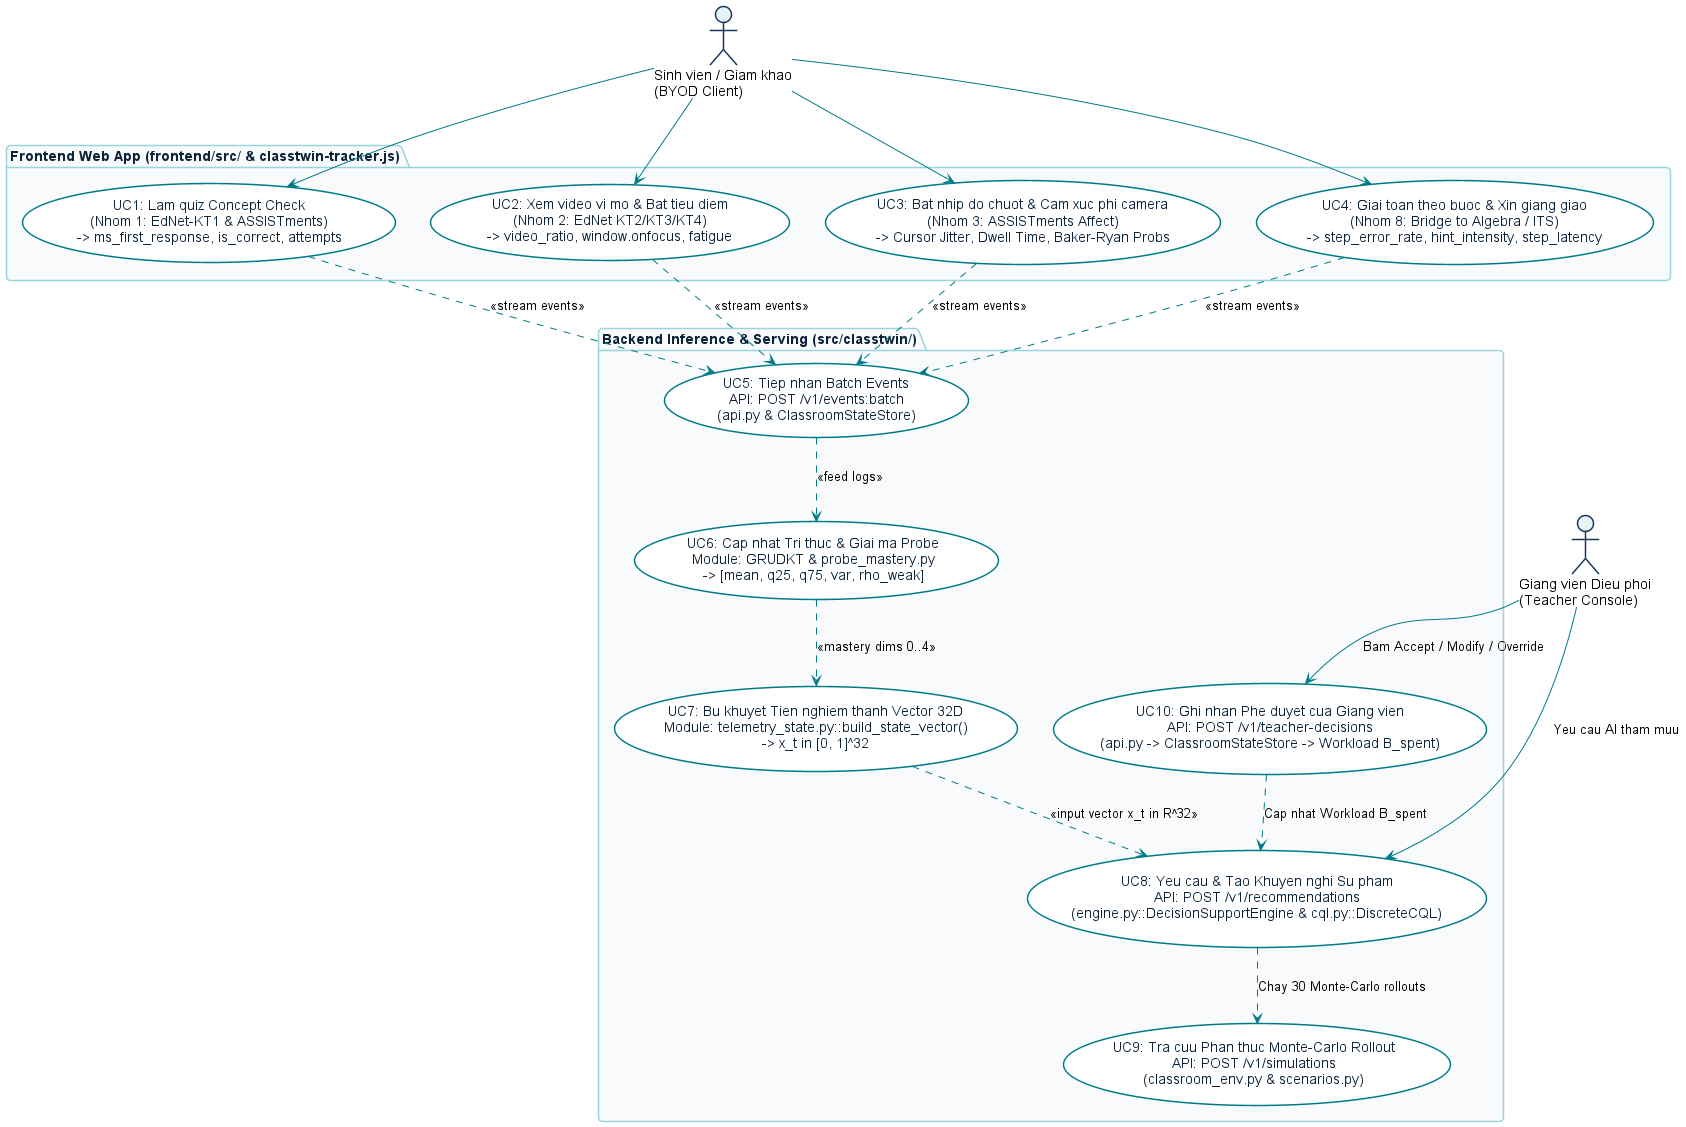
\includegraphics[width=0.92\textwidth]{diagrams/usecases_actors.png}
  \caption{Sơ đồ Tác nhân (Actors) và Ca sử dụng (Use Cases) Ánh xạ Module ClassTwin}\label{fig:usecases}
\end{figure}

\begin{itemize}
  \item \textbf{Phân hệ Frontend Client (\texttt{frontend/src/} \& \texttt{classtwin-tracker.js}):}
  \begin{itemize}
    \item \textbf{UC1 (Nhóm 1): Làm quiz Concept Check:} Đo thời gian do dự trước cú chạm đầu tiên (\texttt{ms\_first\_response}) và tính đúng/sai $y \in \{0, 1\}$ (Tương thích EdNet-KT1 \& ASSISTments).
    \item \textbf{UC2 (Nhóm 2): Xem video vi mô \& Bắt tiêu điểm:} Theo dõi sự kiện HTML5 video (\texttt{play/pause/seek}), cờ \texttt{window.onfocus} và độ mệt mỏi nhận thức (Tương thích EdNet KT2/3/4).
    \item \textbf{UC3 (Nhóm 3): Bắt nhịp độ chuột \& Cảm xúc Baker-Ryan:} Lấy mẫu tọa độ chuột/chạm mỗi 100ms, tính chỉ số rung giật Cursor Jitter và suy diễn 4 xác suất tâm lý (Tương thích ASSISTments with Affect).
    \item \textbf{UC4 (Nhóm 8): Giải toán theo bước \& Xin giàn giáo:} Ghi nhận tỷ lệ sai sót từng bước giải nhỏ (\texttt{step\_error\_rate}) và cường độ bấm xin gợi ý (\texttt{hint\_intensity}) (Tương thích Bridge to Algebra).
  \end{itemize}
  \item \textbf{Phân hệ Backend Inference (\texttt{src/classtwin/}):}
  \begin{itemize}
    \item \textbf{UC5:} Tiếp nhận dòng sự kiện qua API \texttt{POST /v1/events:batch} (\texttt{api.py} nạp vào \texttt{ClassroomStateStore}).
    \item \textbf{UC6:} Cập nhật mạng nơ-ron hồi quy \texttt{GRUDKT} (\texttt{gru\_dkt.py}) và giải mã Probe Mastery qua \texttt{probe\_mastery.py}.
    \item \textbf{UC7:} Ghép nối vector trạng thái 32 chiều qua hàm \texttt{build\_state\_vector()} (\texttt{data/telemetry\_state.py}).
    \item \textbf{UC8:} Khởi tạo tham mưu sư phạm qua API \texttt{POST /v1/recommendations} (\texttt{DecisionSupportEngine} trong \texttt{engine.py} kết hợp Q-Network \texttt{DiscreteCQL} trong \texttt{cql.py}).
    \item \textbf{UC9:} Dự báo phản thực Monte-Carlo qua API \texttt{POST /v1/simulations} (\texttt{ClassroomDigitalTwinEnv} trong \texttt{classroom\_env.py}).
    \item \textbf{UC10:} Ghi nhận quyết định phê duyệt của giảng viên qua API \texttt{POST /v1/teacher-decisions} (\texttt{api.py} cập nhật ngân sách tải $B_{spent}$).
  \end{itemize}
\end{itemize}

% =========================================================================
% MỤC 3: LUỒNG SỰ KIỆN THỜI GIAN THỰC (PLANTUML 2)
% =========================================================================
\section{Luồng Sự Kiện Thời Gian Thực (Real-Time Sequence Flow)}\label{sec:sequence}

Hình~\ref{fig:sequence} mô tả chi tiết trình tự gọi hàm và trao đổi bản tin giữa Client, Gateway API, các Estimator mạng nơ-ron, Policy CQL và Giảng viên theo đúng luồng thực thi trong repo:

\begin{figure}[H]
  \centering
  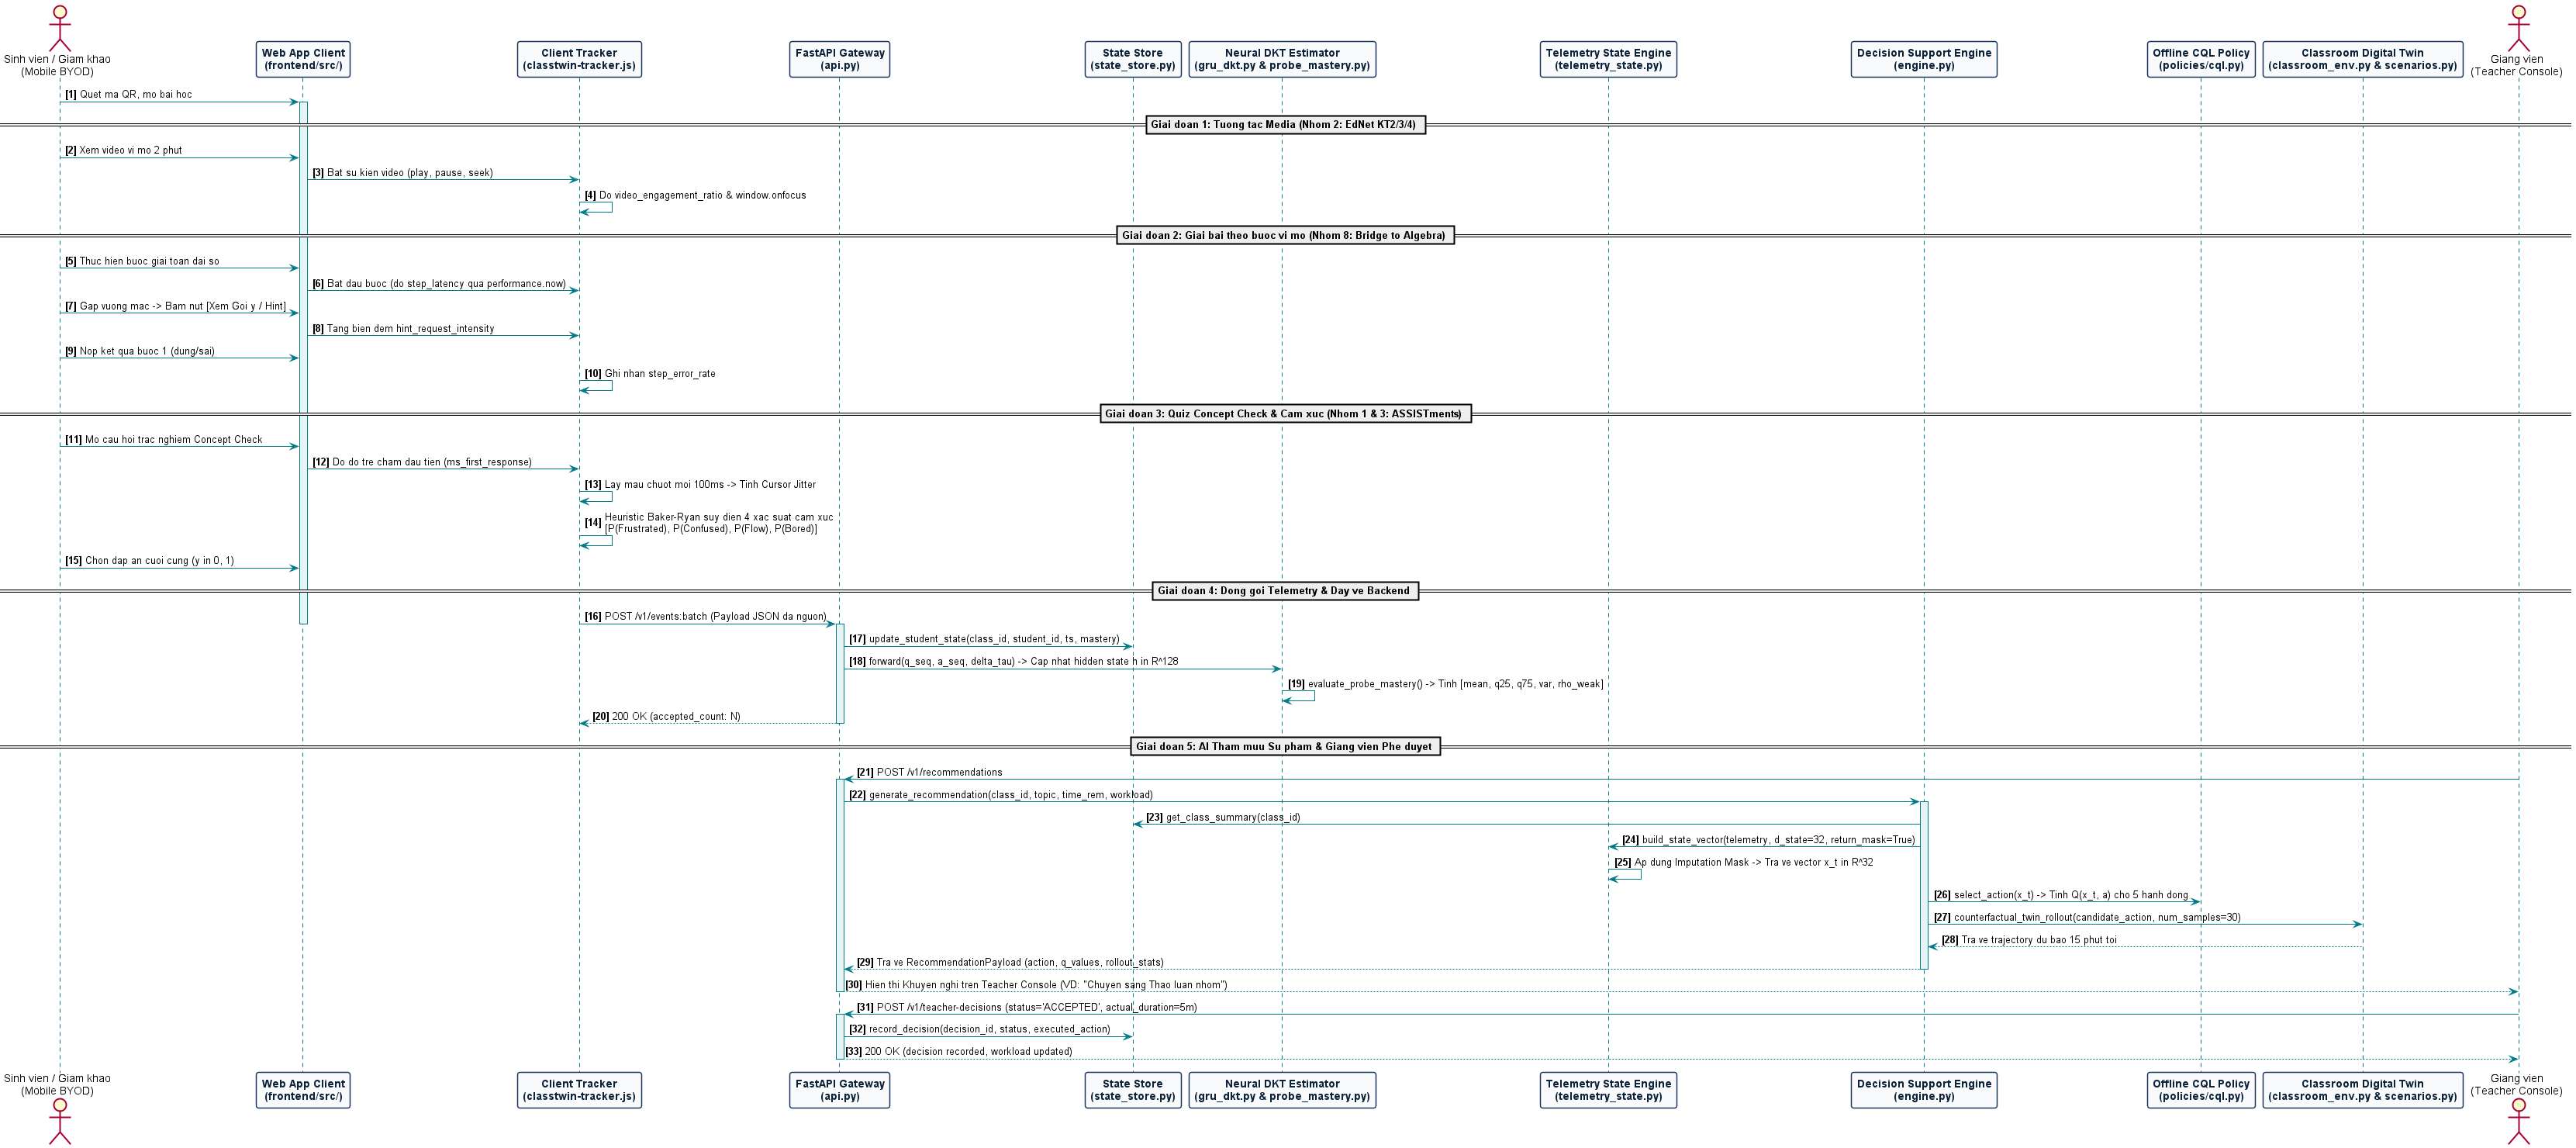
\includegraphics[width=0.92\textwidth]{diagrams/event_sequence.png}
  \caption{Biểu đồ Tuần tự (Sequence Diagram) Luồng Gọi Hàm và Trao Đổi API Thời Gian Thực}\label{fig:sequence}
\end{figure}

Quy trình tuần tự gồm 5 giai đoạn khép kín:
\begin{enumerate}
  \item \textbf{Giai đoạn 1 (Media -- Nhóm 2):} Học sinh xem video vi mô $\implies$ \texttt{classtwin-tracker.js} bắt các sự kiện đa phương tiện, tính tỷ lệ gắn kết media (\texttt{video\_engagement\_ratio}) và giám sát \texttt{window.onfocus}.
  \item \textbf{Giai đoạn 2 (Step Solver -- Nhóm 8):} Học sinh giải toán chia bước $\implies$ \texttt{classtwin-tracker.js} ghi nhận thời gian giải bước 1 qua \texttt{performance.now()} và số lần bấm xin trợ giúp (\texttt{hint\_request\_intensity}).
  \item \textbf{Giai đoạn 3 (Concept Check \& Affect -- Nhóm 1 \& 3):} Học sinh làm quiz trắc nghiệm $\implies$ Tracker đo độ do dự trước lựa chọn đầu tiên (\texttt{ms\_first\_response}), lấy mẫu tọa độ chuột tính Jitter $\implies$ suy diễn xác suất cảm xúc Baker-Ryan.
  \item \textbf{Giai đoạn 4 (Ingestion \& Estimation):} Tracker gửi gói tin JSON tới endpoint \texttt{POST /v1/events:batch}. \texttt{api.py} lưu vào \texttt{ClassroomStateStore}, nạp vào mạng \texttt{GRUDKT} cập nhật $\mathbf{h}_{i, t} \in \mathbb{R}^{128}$ và giải mã phân vị năng lực lớp.
  \item \textbf{Giai đoạn 5 (AI Recommendation \& Teacher Feedback):} Teacher Console gọi \texttt{POST /v1/recommendations}. \texttt{DecisionSupportEngine} gọi \texttt{build\_state\_vector()} để nạp $\mathbf{x}_t \in \mathbb{R}^{32}$ vào mạng \texttt{DiscreteCQL}, kết hợp chạy 30 mẫu mô phỏng Monte-Carlo qua \texttt{counterfactual\_twin\_rollout()}. Giảng viên bấm nút **Accept** $\implies$ gọi \texttt{POST /v1/teacher-decisions} để chốt hành động và trừ ngân sách công sức giảng viên.
\end{enumerate}

% =========================================================================
% MỤC 4: LUỒNG DỮ LIỆU VÀ ÁNH XẠ METRICS SANG 4 DATASETS (PLANTUML 3)
% =========================================================================
\section{Luồng Dữ Liệu Phân Tầng \texorpdfstring{\&}{và} Bản Đồ Ánh Xạ Datasets}\label{sec:dataflow}

Hình~\ref{fig:dataflow} thể hiện cấu trúc 5 tầng chuyển hóa dữ liệu từ thao tác vi mô ở trình duyệt đến các module xử lý nội bộ trong repo:

\begin{figure}[H]
  \centering
  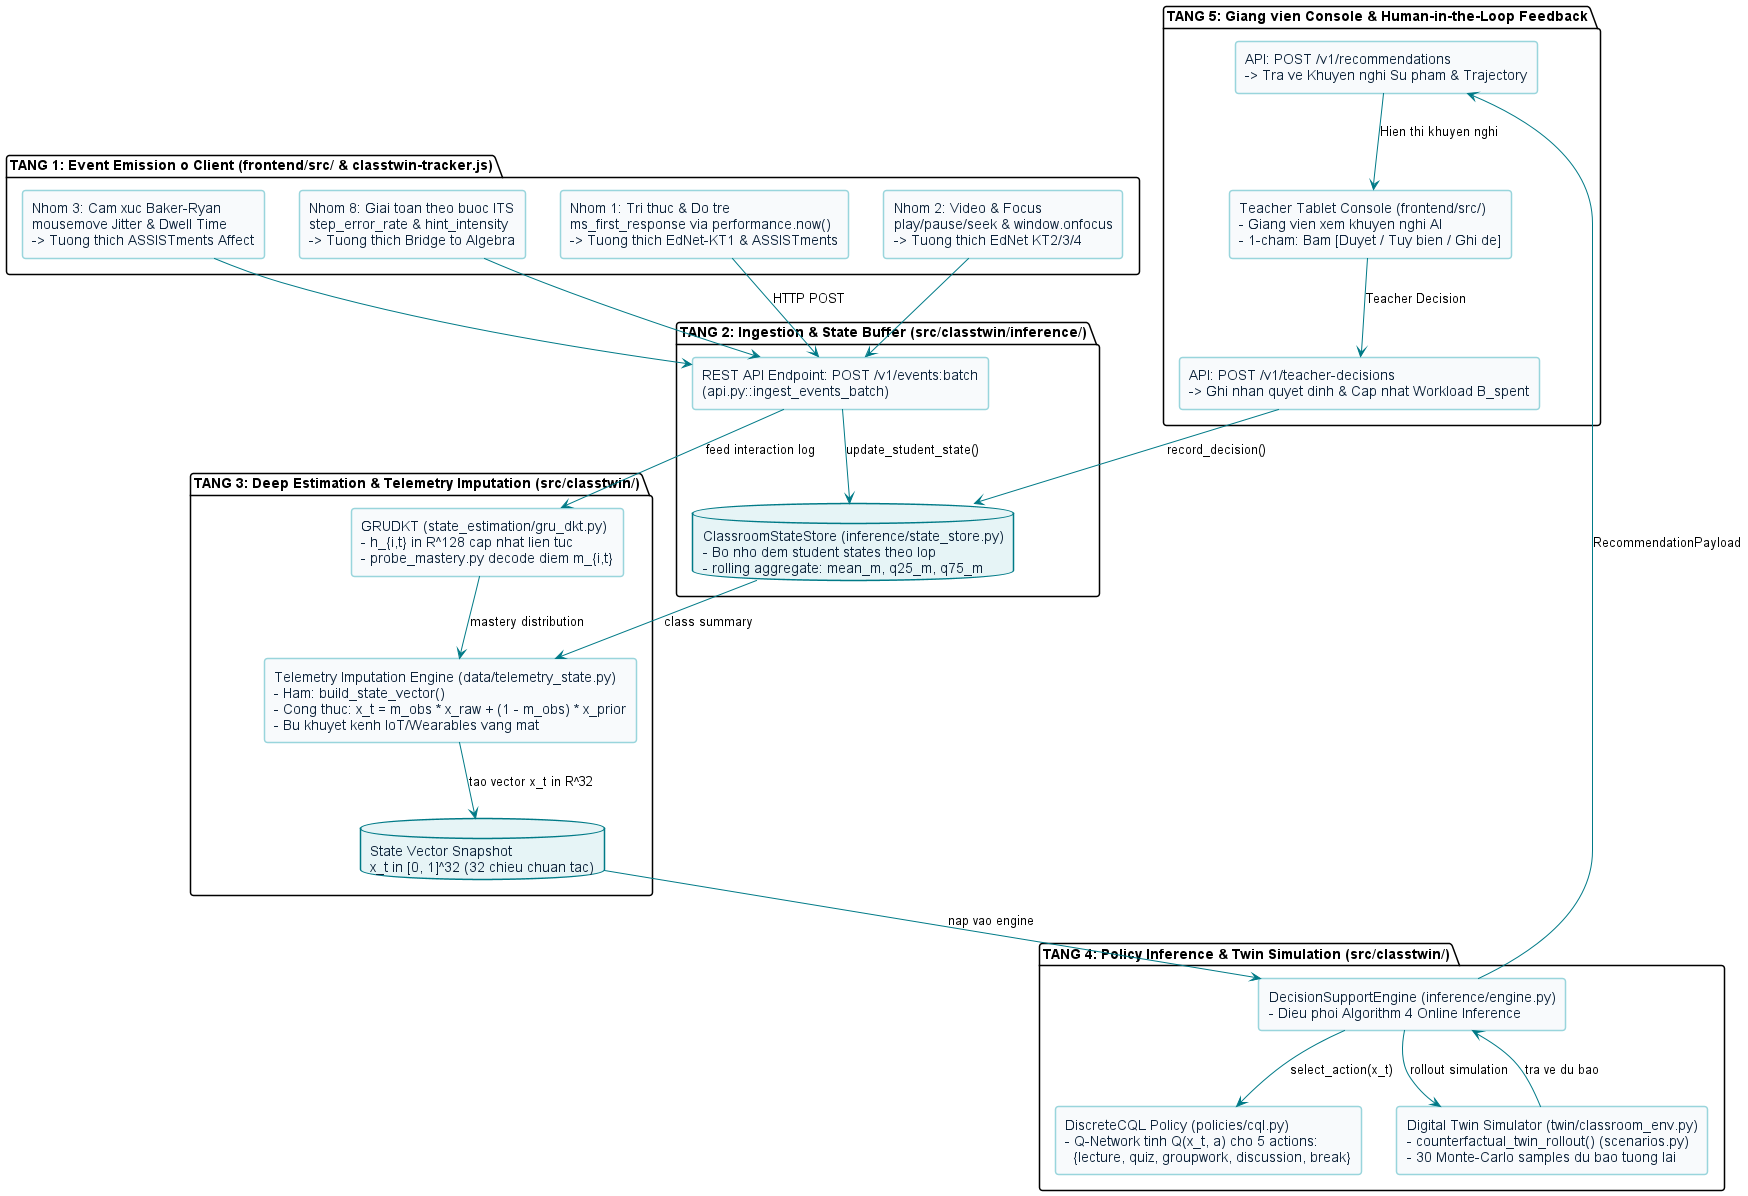
\includegraphics[width=0.92\textwidth]{diagrams/data_flow.png}
  \caption{Sơ đồ Luồng Dữ liệu Phân tầng (Data Flow) và Các Module Xử lý trong Repo}\label{fig:dataflow}
\end{figure}

Bảng~\ref{tab:mapping-datasets-4groups} tổng hợp chi tiết mối liên kết hữu cơ giữa các trường đo đạc được trên Web App giả lập với 4 bộ dữ liệu học thuật quốc tế tương ứng trong ClassTwin:

\begin{table}[H]
  \centering\footnotesize
  \caption{Bản đồ đối chiếu chi tiết 4 Nhóm Viễn trắc Thực địa với 4 Bộ Dữ liệu Học thuật}\label{tab:mapping-datasets-4groups}
  \begin{tabularx}{\linewidth}{p{2.2cm} p{3.2cm} p{3.8cm} X}
    \toprule
    \textbf{Nhóm Viễn trắc} & \textbf{Trường Dữ liệu Thu thập} & \textbf{Phương thức Đo lường (Client JS)} & \textbf{Tương thích Dataset \& Cột Dữ liệu Gốc} \\
    \midrule
    \textbf{Nhóm 1: Tri thức} (Dims 0--4) & \texttt{is\_correct} ($y_{i, t}$), \texttt{ms\_first\_response}, \texttt{probe\_mastery} & Đo bằng \texttt{performance.now()} tính từ lúc mở câu hỏi đến khi chạm đáp án; giải mã GRU-DKT & \textbf{EdNet-KT1} (\texttt{user\_answer}, \texttt{elapsed\_time}) và \textbf{ASSISTments} (\texttt{correct}, \texttt{ms\_first\_response}). \\
    \addlinespace
    \textbf{Nhóm 2: Media} (Dims 5--7) & \texttt{video\_ratio}, \texttt{mean\_attention}, \texttt{fatigue\_rate} & Bắt sự kiện video HTML5 (\texttt{play/pause/seek}) và theo dõi cờ \texttt{document.hidden} & \textbf{EdNet KT2/KT3/KT4} (\texttt{action\_type}, \texttt{cursor\_time}, chuỗi tương tác đa phương tiện). \\
    \addlinespace
    \textbf{Nhóm 3: Cảm xúc} (Dims 8--11) & $P(\text{Frust})$, $P(\text{Conf})$, $P(\text{Flow})$, $P(\text{Bored})$ & Lấy mẫu tọa độ chuột/chạm mỗi 100ms; tính độ gấp khúc Jitter $\mathcal{J}$ và thời gian dừng thao tác & \textbf{ASSISTments with Affect} (\texttt{Avg\_conf(FRUSTRATED)}, \texttt{Avg\_conf(CONFUSED)}, v.v.). \\
    \addlinespace
    \textbf{Nhóm 8: ITS Step} (Dims 25--27) & \texttt{step\_error\_rate}, \texttt{hint\_intensity}, \texttt{step\_latency} & Đếm số lần bấm trợ giúp từng bước giải; ghi nhận kết quả ở lần thực hiện bước đầu tiên & \textbf{Bridge to Algebra} (\texttt{Step Name}, \texttt{Step Duration (sec)}, \texttt{Correct First Attempt}, \texttt{Hints}). \\
    \bottomrule
  \end{tabularx}
\end{table}

% =========================================================================
% MỤC 5: ĐẶC TẢ MÃ NGUỒN TRIỂN KHAI PHÍA CLIENT (TRACKER JS)
% =========================================================================
\section{Đặc Tả Mã Nguồn Triển Khai Client-Side Tracker}\label{sec:client-code}

Đoạn mã JavaScript thuần sau đây tích hợp đồng thời việc đo đạc của cả 4 nhóm (1, 2, 3, 8), sẵn sàng nhúng trực tiếp vào Web App giả lập của nhóm:

\begin{lstlisting}[language=JavaScript, caption={Đoạn mã classtwin-tracker.js tích hợp trọn vẹn 4 nhóm chỉ số 1, 2, 3, 8}]
// classtwin-tracker.js - Telemetry Handler toan dien cho 4 nhom
(function() {
  let sessionStart = performance.now();
  let stepLatencies = [], stepErrors = 0, stepHints = 0, totalSteps = 0;
  let mouseHistory = [], blurStart = null, totalBlurMs = 0;
  let videoWatchSec = 0, videoTotalSec = 120; // Video bai giang 2 phut

  // [NHOM 2] Lang nghe su kien Video Media & Focus
  document.addEventListener("visibilitychange", () => {
    if (document.hidden) blurStart = performance.now();
    else if (blurStart) { totalBlurMs += (performance.now() - blurStart); blurStart = null; }
  });
  const videoElem = document.getElementById("lecture-video");
  if (videoElem) {
    videoElem.addEventListener("timeupdate", () => { videoWatchSec = videoElem.currentTime; });
  }

  // [NHOM 3] Lay mau chuot moi 100ms de tinh Jitter & Cam xuc Baker-Ryan
  window.addEventListener("mousemove", (e) => {
    const now = performance.now();
    mouseHistory.push({ x: e.clientX, y: e.clientY, t: now });
    if (mouseHistory.length > 25) mouseHistory.shift();
  });

  function calculateBakerRyanAffect() {
    let jitter = 1.0;
    if (mouseHistory.length >= 3) {
      let totalDist = 0;
      for (let i = 1; i < mouseHistory.length; i++) {
        totalDist += Math.hypot(mouseHistory[i].x - mouseHistory[i-1].x, mouseHistory[i].y - mouseHistory[i-1].y);
      }
      let directDist = Math.hypot(mouseHistory[mouseHistory.length-1].x - mouseHistory[0].x, mouseHistory[mouseHistory.length-1].y - mouseHistory[0].y);
      jitter = directDist > 10 ? (totalDist / directDist) : 1.0;
    }
    const pFrustrated = Math.min(0.85, Math.max(0.05, 0.10 + (jitter > 3.2 ? 0.35 : 0.0)));
    const pBored = Math.min(0.85, Math.max(0.05, 0.12 + (totalBlurMs > 6000 ? 0.40 : 0.0)));
    const pConfused = Math.min(0.85, Math.max(0.05, 0.15 + (jitter > 2.0 && jitter <= 3.2 ? 0.25 : 0.0)));
    const pConcentrating = Math.max(0.1, 1.0 - (pFrustrated + pBored + pConfused));
    return { pFrustrated, pConfused, pConcentrating, pBored };
  }

  // [NHOM 8] Lang nghe cac buoc giai toan vi mo (Cognitive Tutor)
  window.recordStepAction = function(stepIndex, isCorrect, requestedHint) {
    totalSteps++;
    if (!isCorrect) stepErrors++;
    if (requestedHint) stepHints++;
  };

  // [NHOM 1] Dong goi va gui Telemetry khi nop bai Quiz tong ket
  window.submitFullTelemetry = function(studentId, qId, isQuizCorrect, quizLatencyMs) {
    const affect = calculateBakerRyanAffect();
    const payload = {
      events: [{
        student_id: studentId || "stu_evaluator",
        class_id: "class_scic_live",
        question_id: qId,
        is_correct: Boolean(isQuizCorrect),
        ms_first_response: Math.round(quizLatencyMs),
        video_ratio: Math.min(1.0, videoWatchSec / videoTotalSec),
        step_error_rate: totalSteps > 0 ? (stepErrors / totalSteps) : 0.28,
        hint_intensity: totalSteps > 0 ? (stepHints / totalSteps) : 0.20,
        prob_frustrated: affect.pFrustrated,
        prob_confused: affect.pConfused,
        prob_concentrating: affect.pConcentrating,
        prob_bored: affect.pBored,
        event_ts_ms: Date.now()
      }],
      schema_version: "v1.0"
    };
    fetch("/v1/events:batch", {
      method: "POST",
      headers: { "Content-Type": "application/json" },
      body: JSON.stringify(payload)
    });
  };
})();
\end{lstlisting}

% =========================================================================
% MỤC 6: KỊCH BẢN TRÌNH DIỄN 5 PHÚT
% =========================================================================
\section{Kịch Bản Trình Diễn Thực Tế 5 Phút Dành Cho Hội Đồng SCIC 2026}\label{sec:kich-ban-demo}

\begin{stepbox}[{Kịch Bản Trình Diễn Live Đột Phá 5 Phút Trước Ban Giám Khảo}]
\begin{itemize}
  \item \textbf{Phút 1: Quét QR \& Trải nghiệm Video (Nhóm 2):} Giám khảo quét mã QR trên màn hình chiếu, mở Web App giả lập. Giám khảo xem thử 1 video vi mô 30 giây. Màn hình lớn của nhóm lập tức hiển thị chỉ số \texttt{video\_engagement\_ratio} và mức chú ý tăng vọt theo thời gian thực.
  \item \textbf{Phút 2: Trải nghiệm Giải bài theo bước (Nhóm 8):} Giám khảo thực hiện giải bài toán chia bước, thử bấm nút \textit{"Xem Gợi ý / Hint"}. Dashboard lập tức nhảy số chỉ số \texttt{hint\_request\_intensity} và tỷ lệ lỗi bước giải, chứng minh hệ thống đang theo vết nhận thức vi mô của từng cá nhân.
  \item \textbf{Phút 3: Concept Check \& Biểu cảm Baker-Ryan (Nhóm 1 \& 3):} Giám khảo làm câu hỏi kiểm tra nhanh, cố tình rê chuột do dự hoặc chuyển tab. Mô hình Baker-Ryan lập tức ước lượng xác suất $P(\text{Confused})$ hoặc $P(\text{Bored})$ tăng lên; đồng thời mạng GRU-DKT giải mã Probe Mastery và cập nhật phân vị $\bar{m}, Q_{25}, Q_{75}$ của cả lớp.
  \item \textbf{Phút 4: AI Khuyến Nghị Chính Sách Offline CQL:} Thuật toán Offline RL phân tích toàn diện vector 32 chiều (kết hợp các chiều 1, 2, 3, 8 thu được với bộ bù khuyết tiên nghiệm). Nhận thấy học sinh đang bối rối và phân hóa trình độ, AI đề xuất can thiệp: \textbf{"Chuyển sang Thảo luận nhóm đôi bạn cùng tiến (Groupwork 5 phút)"}.
  \item \textbf{Phút 5: Giảng viên Phê duyệt \& Trạng thái Lớp Tối ưu:} Thuyết trình viên cầm máy tính bảng bấm nút **Accept** trên Teacher Console. Màn hình lớp học tự động chuyển sang chế độ thảo luận nhóm, các chỉ số tri thức phục hồi, hoàn thành xuất sắc chu trình sư phạm đóng kín.
\end{itemize}
\end{stepbox}

\end{document}
